% ##############################################################################
% ##############################################################################
% #######   PLANTILLA FODAMI CAIM-CAIFE 2025                            ######## 
% #######   Creado con TeXstudio v 4.8.6   (c/archivo .cls)             ########
% #######   Autores: Equipo FIE - EAS|EAH|SEM                           ########
% ##############################################################################
\documentclass[a4paper]{fodami}        % customizado en archivo .cls    ########
%\usepackage{showframe}                % show layout de página (opt)    ########
% ##############################################################################
% ##############################################################################

\usepackage{xcolor}
\newcommand{\mr}[1]{\textcolor{blue}{#1}}

% ---------- TÍTULO ------------------------------------------------------------
\title{\textbf{INTRODUCCIÓN TEMPRANA DE LA MECÁNICA COMPUTACIONAL EN CURSOS DE ELECTROSTÁTICA Y MECÁNICA ANALÍTICA}}

% ---------- AUTORES -----------------------------------------------------------
\author[1*]  {\textbf{Víctor A. Bettachini}}
\author[2]{\textbf{Mariano A. Real}}
\author[3]{\textbf{Edgardo Palazzo}}

% ---------- AFILIACIÓN --------------------------------------------------------
\setlength\parindent{0pt}
\affil[1]{Departamento de Ingeniería e Investigaciones Tecnológicas, Universidad Nacional de La Matanza (DIIT UNLaM), Florencio Varela 1903, B1754JEC San Justo,Buenos Aires, Argentina.}
% \affil[1]{Departamento Académico de Mecánica, UTN - Facultad Regional Santa Fe, Lavaisse 610, 3000 Santa Fe, Argentina.}

\affil[2]{Instituto de Calidad Industrial, Universidad Nacional de San Martín - Instituto Nacional de Tecnología Industrial (INCALIN UNSaM-INTI), Av. General Paz 5445, B1684EFA Villa Martelli, Buenos Aires, Argentina.}

\affil[3]{Departamento de Materias Básicas, Universidad Tecnológica Nacional - Facultad Regional Avellaneda (UTN FRA), Ramón Franco 5050, B1876ABY Villa Domínico, Buenos Aires, Argentina}

\affil[*]{Email: vbettachini@unlam.edu.ar}


% ##############################################################################
\begin{document}
\date{}

% ########## ENCABEZAMIENTOS y PIE #############################################
\renewcommand{\headrulewidth}{0pt} \renewcommand{\footrulewidth}{0pt}
\pagestyle{fancy}
\fancyhead{}
\fancyhead[C]{
	
\includegraphics[width=11.5cm]{imagenes/logoFODAMICAIMCAIFE.pdf}
	\noindent
	{\color{lightgray} \rule{\linewidth}{0.14cm}}
}
\fancyfoot{}
\fancyfootoffset[L]{-4cm}
\fancyfoot[L]{\footnotesize \flushleft \emph{IX CAIM 2025 - Noveno Congreso Argentino de Ingeniería Mecánica \\  
	IV CAIFE 2025 - Cuarto Congreso Argentino de Ingeniería Ferroviaria} \\
	\url{www.fie.undef.edu.ar/caimcaife2025} |  \href{mailto:caimcaife2025@fie.undef.edu.ar}{caimcaife2025@fie.undef.edu.ar}}
\setlength{\parskip}{8pt}
% ##############################################################################
	
\maketitle
\thispagestyle{fancy}

% ---------- RESUMEN -----------------------------------------------------------
\section*{
	\begin{center}
		RESUMEN
	\end{center}}
\vspace{-1.0cm}

Este trabajo presenta dos experiencias educativas que integran herramientas computacionales en la enseñanza de física para ingeniería, abordando desafíos comunes en entornos con recursos limitados.

La primera propuesta desarrolló un curso de mecánica analítica basado en Python, utilizando Jupyter notebooks y un enfoque de aula invertida.
Los estudiantes resuelven ecuaciones de Euler-Lagrange mediante bibliotecas como SymPy y SciPy, centrándose en el modelado físico y evitando simplificaciones pedagógicas.
El curso, disponible en GitHub, ha demostrado eficacia en grupos pequeños, aunque requiere adaptaciones para escalabilidad.

La segunda experiencia aplicó metodologías similares en electrostática, permitiendo a alumnos analizar distribuciones de carga continuas mediante cálculos numéricos en Google Colaboratory.
Los resultados destacan una mayor comprensión conceptual sin depender de técnicas matemáticas avanzadas.

Ambos casos subrayan cómo la programación accesible (Python) y entornos interactivos (Jupyter) optimizan el tiempo en clase, priorizando el análisis sobre cálculos repetitivos, y ofrecen soluciones viables para instituciones con restricciones presupuestarias o logísticas.
Estas estrategias, replicables y de código abierto, podrían extenderse a otras áreas de la física e ingeniería, potenciando el aprendizaje activo en contextos diversos.


\textit{\textbf{Palabras claves}: Enseñanza; Ingeniería Mecánica; Código; Inteligencia artificial.}



% ---------- CUERPO del DOCUMENTO ----------------------------------------------
\newpage
\onehalfspacing
\setlength{\parskip}{0pt}
% ------------------------------------------------------------------------------

\section{INTRODUCCIÓN}

\subsection{Las asignaturas de física, puente entre asignaturas básicas y específicas de la ingeniería mecánica}
En las carreras de ingeniería mecánica las asignaturas de física integran lo dictado en las de matemática para proveer herramientas a aquellas específicas de la carrera.
En una asignatura del tercer año de la Universidad Nacional de La Matanza (UNLaM) se dicta el formalismo Lagrangiano para el cálculo de esfuerzos y dinámica de sistemas de cuerpos, con vistas a aplicarle en las asignaturas destinadas a la mecánica de fluidos, el estudio de vibraciones y la dinámica de elementos de máquinas (Figura \ref{fig:correlativasUNLaM}).

\begin{figure}[ht]
	\centering
	\begin{subfigure}[b]{0.5\textwidth}
		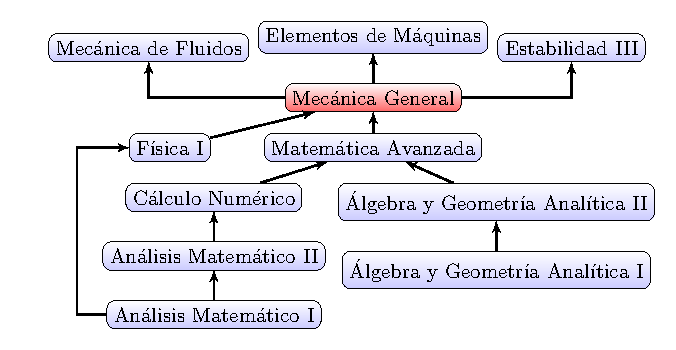
\includegraphics[width=\textwidth]{../figuras/correlativas_2.pdf}
		\caption{
			La asignatura de mecánica analítica de la UNLaM oficia de umbral hacia las específicas de la carrera.  
		}
		\label{fig:correlativasUNLaM}
	\end{subfigure}
	\hfill
	\begin{subfigure}[b]{0.45\textwidth}
		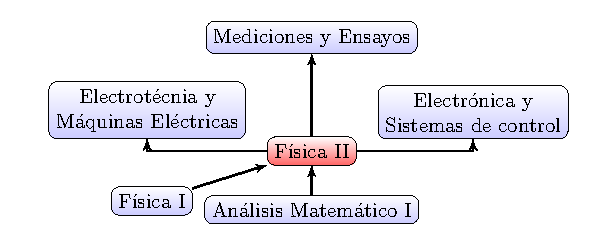
\includegraphics[width=\textwidth]{../figuras/utn_fra_ingMec_correlativasF2_2.pdf}
		\caption{
			En UTN FRA la primera asignatura con temática de electromagnetismo abre el camino a otras en que esta se aplica a dispositivos industriales de electrotecnia y electrónica.
			Se muestran solo las correlativas con aplicación inmediata de conceptos de electromagnetismo. 
		}
		\label{fig:correlativasUTN}
	\end{subfigure}
	\caption{
		En las carreras de ingeniería mecánica las asignaturas de física ofician de puente entre las asignaturas básicas y aquellas con la temática propia de la carrera.
	}
	\label{fig:correlatividades}
\end{figure}

En la Facultad Regional Avellaneda de la Universidad Tecnológica Nacional (UTN FRA), en una asignatura aún más temprana (segundo año), se dictan los rudimentos de electromagnetismo que se aplican en las asignaturas inmediatamente correlativas que tratan ensayos y mediciones en la industria, así como los fundamentos del funcionamiento de dispositivos tanto electrotécnicos como de electrónica industrial (Figura \ref{fig:correlativasUTN}).


\subsection{La mecánica computacional como herramienta para evitar saltos de complejidad entre asignaturas}

Usualmente, las modelizaciones que se trabajan en las asignaturas de física son ``de juguete'', en los términos de que difieren en demasía respecto a dispositivos que puede tener aplicación industrial.
Como evidencia la Figura \ref{fig:correlatividades}, estos son el objeto de las siguientes asignaturas que cursan los alumnos, lo que lleva a un ``salto de complejidad''. %ue usualmente resulta en que en dichas asignaturas se recurre a  desaprovecha lo aprendido en las asignaturas básicas al      

Hay variadas limitaciones para que en clases de las asignaturas de física se modelen sistemas físicos realistas.
Puede que su complejidad requiera obtener analíticamente extensos sistemas de ecuaciones integro-diferenciales, tal es el caso del curso de mecánica analítica de la UNLaM, lo que demandaría en papel o pizarrón un tiempo que excede el de la clase.
O puede que los alumnos no han cursado aún las asignaturas de matemática para resolver analíticamente tales ecuaciones, como sucede en la asignatura de electromagnetismo de la UTN FRA.

Ambas falencias pueden suplirse introduciendo en las asignaturas de física la mecánica computacional.
Esta disciplina conjuga la matemática, las distintas ramas de la física y herramientas de ciencias de la computación para explicar la dinámica de sistemas físicos de diversa composición ante muy variados forzantes externos.
Entendemos que una exitosa explotación de esta herramienta en las primeras asignaturas de la carrera de ingeniería mecánica requiere se cumplan dos condiciones.
La primera, desplazar el pizarrón y papel como soportes en que se expresan tanto docentes como alumnos.
Y la segunda, no depender de un software específico que limite la posibilidad de adaptar las soluciones y utilizar el código como una herramienta de trabajo. 



\subsection{Pizarrón y papel, foco de las clases en la tercera década del siglo XXI}	

En la tercera década del siglo XXI los cursos de ingeniería de las universidades latinoamericanas tienen aún como herramientas centrales el papel y el pizarrón.
Introducido en el siglo XIX, este último siguió siendo el foco del aula en los siglos subsiguientes.
La Figura \ref{fig:oldSchool} podría corresponder a un aula contemporánea.
Desde entonces la metodología de la clase se resumen en que el docente presenta un tema con anotaciones en el pizarrón, los alumnos toman apuntes en papel, luego realizan la ejercitación, que el docente puede luego corregir en el mismo soporte.

\begin{figure}[ht]
	\centering
	\begin{subfigure}[b]{0.395\textwidth}
	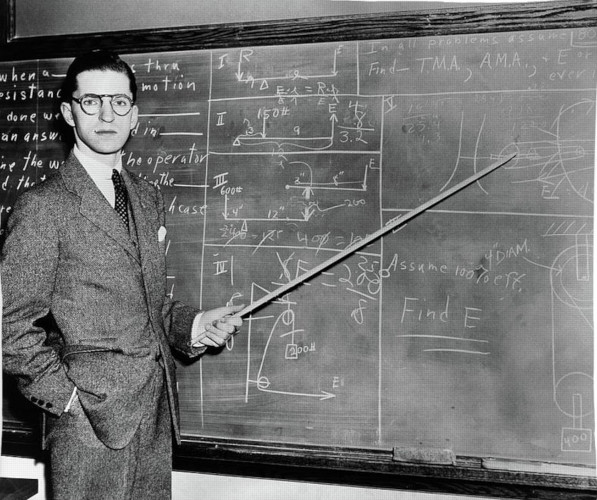
\includegraphics[width=\textwidth]{../figuras/1930s-1940s-man-teacher-professor-vintage-images.jpg}
	\caption{
		Pizarrón de una clase de física, c. 1930.
		}
	\label{fig:oldSchool}
	\end{subfigure}
	\hfill
	\begin{subfigure}[b]{0.59\textwidth}
	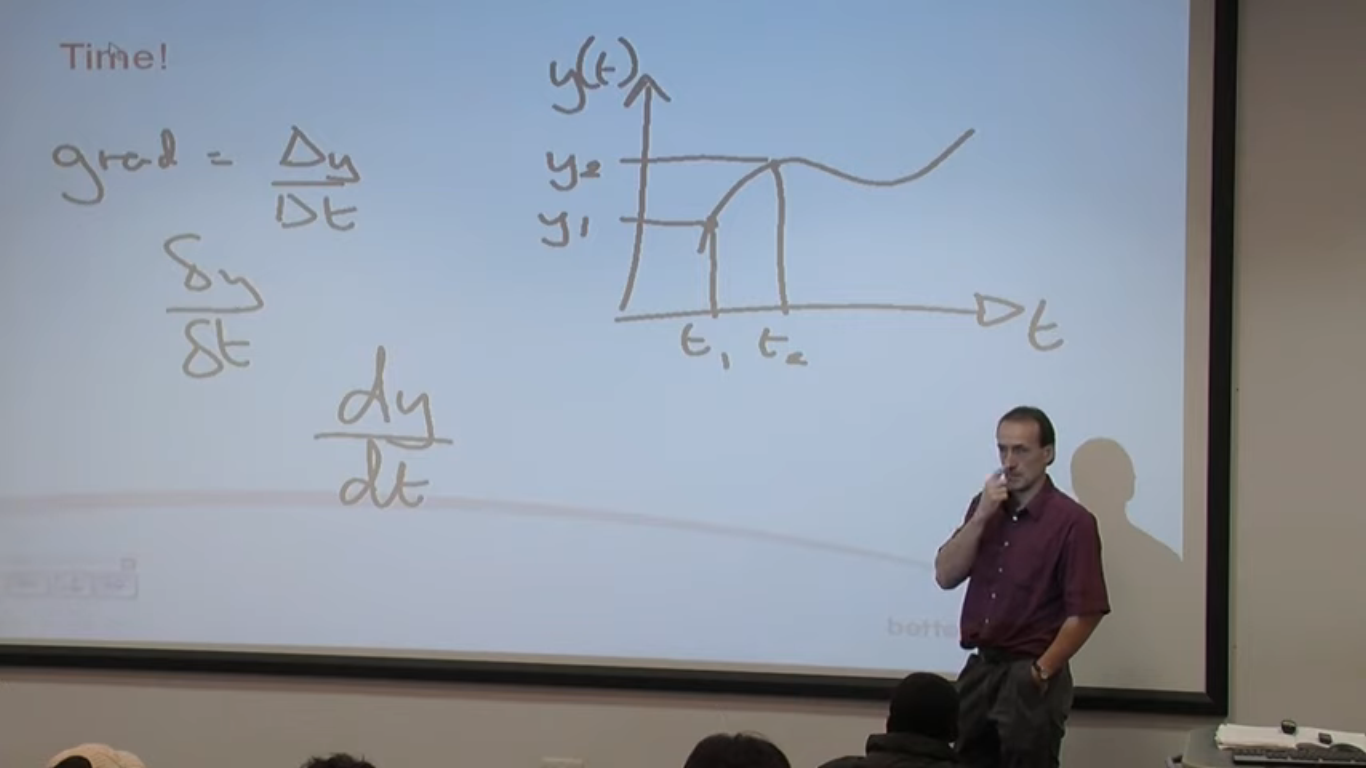
\includegraphics[width=\textwidth]{../figuras/systemsEngineering.png}
	\caption{
		Proyección de una clase de análisis matemático, c. 2010.
		}
	\label{fig:oldSchool2010}
	\end{subfigure}
	\caption{
		En el s. XXI se hace un uso del pizarrón idéntico a cuando se le introdujo en el aula del s. XIX.
		Si está presente en el aula, la computadora es usualmente un mero substituto de este último.
		}
	\label{fig:tradicional}
\end{figure}

En las últimas décadas del siglo XX se generalizó el uso de computadoras en el aula, aunque los docentes usualmente les reducen a ser una mera herramienta de proyección, que como muestra la Figura \ref{fig:oldSchool2010} excluye a los alumnos de su uso. 
Y ellos, aun cuando realicen sus anotaciones en computadoras portátiles, reproducen aún el mismo esquema del s. XIX, invirtiendo buena parte de su tiempo y atención en transcribir lo mostrado en un pizarrón.

Esta sub explotación en el aula de la inherente capacidad de rápida reproducción de la información digital queda aún más fuera del contexto actual ante la omnipresencia de grandes modelos de lenguaje (LLM) como ChatGPT o DeepSeek, que permiten a los estudiantes obtener una rápida orientación sobre la temática que se está tratando.  
Los formatos papel y pizarrones fuerzan a una transcripción desde y hacia el medio digital para poder hacer provecho de los LLM.
Tal transcripción de sus anotaciones en papel al teléfono o computadora conectadas a internet, sumada al arcaico proceder de tomar apuntes en clase, es sumar una tarea adicional que distrae al alumno del pensamiento creativo que debiera ser el foco de su esfuerzo.

Por estas razones es que en los cursos aquí presentados se busca utilizar el mismo formato digital, tanto para el dictado de lecciones por parte del docente, como para la ejercitación por parte de los alumnos.
Dicho medio no solo es capaz de representar todo el contenido gráfico que puede mostrarse en un pizarrón, incluyendo las ecuaciones integro-diferenciales que modelan cualquier sistema físico a analizar, sino que también permite resolver estas últimas.
Esto abre el camino a utilizar en clase representaciones gráficas precisas de dichos resultados, y en particular de los obtenidos por métodos del cálculo numérico.
% Esto último con el fin de que el alumno pueda poner en práctica la mecánica computacional como una herramienta de trabajo en la asignatura. 



\subsection{El código como herramienta central de la asignatura}

Si nos proponemos hacer mecánica computacional en un curso de grado de ingeniería, puede resultar tentador usar algún paquete de software específico para resolver problemas de física, que permita modelizar y simular sistemas utilizando alguna interfaz gráfica, como Comsol Multiphysics, Ansys o SolidWorks.
O, por el contrario, utilizar un paquete de software más específico de matemática computacional, como Mathematica o Matlab.

Ante este abanico de opciones, no hay que olvidar que las asignaturas de física se ubican al inicio de las carreras de ingeniería mecánica, y el alumno en tal estadío no tiene aún la formación suficiente para comprender en detalle las herramientas de modelización y simulación que ofrecen los paquetes de software específicos de matemática o mecánica computacional.
Entendemos que para que la propuesta pueda ser transversal a las varias temáticas de las múltiples asignaturas correlativas, se debe utilizar una herramienta aún más general. 
Con este supuesto es que se optó por hacer uso de Python, un lenguaje de programación de alto nivel, que además resulta ser abierto y libre, virtudes acordes a las limitaciones de las aulas de nuestras universidades

Para que la implementación de Python sea vista como una continuación de lo aprendido en las asignaturas de matemática, este debe operar el álgebra y análisis simbólico con la misma nomenclatura matemática que se utiliza en el pizarrón.
Para tal fin se hace uso de la biblioteca SymPy \cite{sympy} que permite operar con álgebra simbólica utilizando la nomenclatura matemática habitual.
Esto es fundamental para que el docente pueda intercalar en sus explicaciones cálculos realizados por el código que sean inteligibles para el alumno.

Para capitalizar lo aprendido en asignaturas de cálculo numérico, con el fin de obtener soluciones de las complejas ecuaciones integro-diferenciales generadas con auxilio de SymPy, se recurre a la biblioteca SciPy \cite{2020SciPy-NMeth}.
Tales resultados se representan gráficamente haciendo uso de la biblioteca Matplotlib \cite{Hunter:2007}.


\subsection{Usar código para hacer menos tediosa la matemática no requiere de saber programar}

Es importante recalcar que aprovechar código para estas tareas en una asignatura no implica enseñar a programar.
En ninguno de los casos reportados en este trabajo se busca que el alumno aprenda a modelar algorítmicamente teniendo en cuenta cuestiones de la arquitectura informática de los sistemas que utiliza.
%, lo que sería programar.
% Propongo estos dos cambios (anterior y siguiente) porque me suena un toque condescendiente con el lector ponerlo tan explícito. Es sólo sugerencia.
Por el contrario, solo se requiere que plasmen soluciones a la serie de problemas a través de adaptar código escrito por los docentes, algo que no es más que una mera reutilización de este código.
%, un concepto que se denomina reutilización de código.

El punto de utilizar la herramienta informática es despreocupar a los alumnos del trabajo matemático para centrarlo en los nuevos conceptos propios de la asignatura.
De igual manera que un alumno de secundaria resuelve aritmética con una calculadora de bolsillo tras haberle aprendido en la primaria, nuestros alumnos automatizan lo aprendido en asignaturas anteriores.
Por otra parte, extendemos con un uso sistemático de cálculos simples a la resolución de problemas complejos, que requerirían de cálculos integro-diferenciales que aún no dominan, evitando la posible frustración de un trabajo tan monótono y que en numerosas ocasiones no puede ser concluido, o lo es en forma incorrecta, debido a las dificultades matemáticas \cite{Pekrun2006}.
Esto permite resolver más problemas con retroalimentación inmediata, que se traduce en más práctica para la incorporación de conceptos, trabajando en forma autónoma, reutilizando y adaptando código para experimentar con problemas cada vez más complejos, incluso no solo entre los propuestos en esta materia, atesorando así una herramienta que podrán aprovechar en otros contextos.

Desplazando aún más la idea de que se está pidiendo aprender a programar, el formato digital utilizado no pone en preeminencia el código en lenguaje Python sobre otro material, como el texto, ecuaciones o gráficos generados en forma externa.
Dicho formato son los cuadernos Jupyter, como el que muestra la Figura \ref{fig:jupyter}.

\begin{figure}[ht]
	\centering
	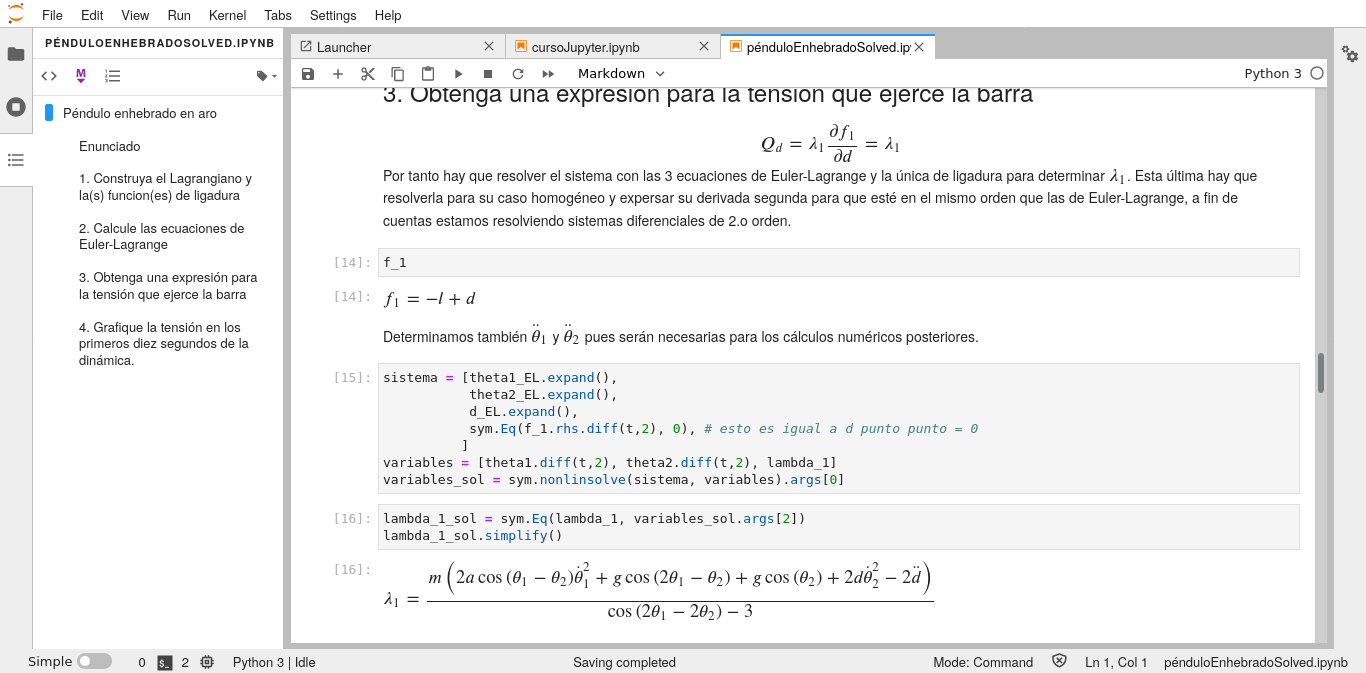
\includegraphics[width=\textwidth]{../figuras/screenshot_JupyterLab.png}
	\caption{
		El docente presenta el tema y los ejemplos en un cuaderno Jupyter, y el alumno puede resolver los ejercicios en una copia de ese cuaderno.
		Tales cuadernos Jupyter permiten intercalar texto, ecuaciones y gráficos generados manualmente con aquellos producidos por el código Python con una nomenclatura matemática estandarizada y gráficos claros.
		}
	\label{fig:jupyter}
\end{figure}

El alumno copia el cuaderno Jupyter provisto por el docente, que contiene no solo el contenido teórico de la lección, sino también el código Python que resuelve un problema de ejemplo.
Modificando ligeramente dicho código puede resolver lo que se le proponen en una guía de ejercicios.
Siendo la copia digital, el alumno es liberado de la tarea de transcribir lecciones, y su esfuerzo durante la clase puede dirigirse a la resolución de los mencionados ejercicios en cuadernos Jupyter individuales.
Estos pueden corregirse por el docente en el mismo formato en que las expresiones matemáticas y gráficos primero están estandarizados y son, por tanto, rápidamente inteligibles.



\subsection{Los recursos están: plataformas en línea}

Se ha argumentado que las universidades públicas latinoamericanas enfrentando restricciones simultáneas de presupuestos ajustados y la necesidad de acomodar los horarios de sus clases a estudiantes que trabajan de día a horarios vespertinos, no cuentan con recursos informáticos para destinar a cursos que no estén directamente relacionados con la informática o la programación 
\cite{vallejo_google_2022}.
Sin embargo, la experiencia del confinamiento por la pandemia de COVID-19 ha demostrado que es posible utilizar plataformas en línea para la enseñanza de asignaturas que no son informáticas.
El uso de tales plataformas solo requieren de una conexión a internet.
El alumno accede a las mismas utilizando una computadora personal, sea en su hogar, en su trabajo o una biblioteca. 
Incluso, en uno de los cursos reportados en este trabajo, el alumnado ha hecho uso de teléfonos inteligentes, no solo para acceder a los cuadernos Jupyter, sino también para editarlos con la finalidad de resolver los ejercicios.

Existen varias plataformas en línea, y de uso gratuito, que permiten la edición de cuadernos Jupyter y ejecutar código Python en ellos, como Google Colaboratory, GitHub Codespaces, Kaggle o CoCalc, entre otras.
Una de las funcionalidades de estas plataformas es que permiten compartir el cuaderno Jupyter con otros usuarios, lo que fomenta entre los alumnos al trabajo colaborativo a distancias, una competencia fundamental en el ámbito laboral actual.
Lo que es tal vez más importante, el docente puede comentar y corregir cuadernos de los alumnos a distancia y en tiempo real, lo que habilita consultas asincrónicas sobre los ejercicios, y no solo sincrónico como en el caso de las clases presenciales.
En estas plataformas los cuadernos con la resolución de ejercicios por parte de los alumnos quedan a resguardo en la cuenta personal de los mismos.
Pueden así servirles de referencia futura para aplicarse en asignaturas posteriores o incluso en su vida profesional.


\section{CURSO DE MECÁNICA ANALÍTICA}

\subsection{Trabajando con dispositivos mecánicos realistas}

La complejidad de la matemática para modelizar sistemas crece rápidamente a medida que se contemplan más factores para hacer del modelo más fiel a los elementos que se presentan el sistema físico real.
Una vez esquematizado el sistema físico, como muestra la Figura \ref{fig:esquema}, se debe calcular la energía potencial y cinética del sistema, así como los momentos de inercia de los cuerpos que lo componen. 
A partir de estos, generar con el formalismo Lagrangiano las ecuaciones para la dinámica y despejar las aceleraciones es una tarea trivial para las funciones de la biblioteca de álgebra simbólica SymPy, como ilustra la Figura \ref{fig:aceleraciones}.

\begin{figure}[ht]
	\centering
	\begin{subfigure}[b]{0.3\textwidth}
		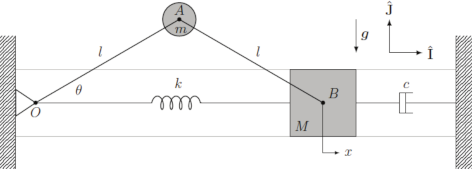
\includegraphics[width = \textwidth]{../figuras/clase7esquema.png}
		\caption{Modelizar posiciones, momentos de inercia para calcular energías potenciales y cinéticas.}
		\label{fig:esquema}
	\end{subfigure}
	\hfill
	\begin{subfigure}[b]{0.4\textwidth}
		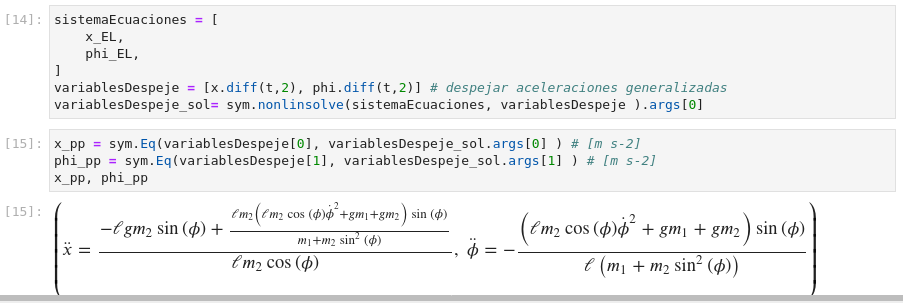
\includegraphics[width = \textwidth]{../figuras/clase4Aceleraciones.png}
		\caption{Generar con formalismo Lagrangiano las ecuaciones diferenciales de la dinámica.}
		\label{fig:aceleraciones}
	\end{subfigure}
	\begin{subfigure}[b]{0.28\textwidth}
		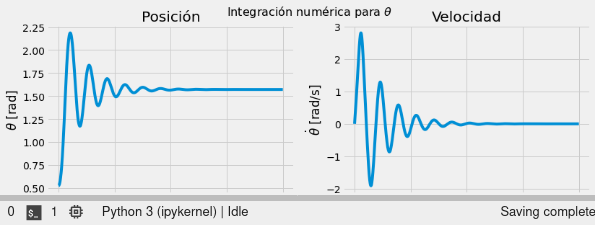
\includegraphics[width = \textwidth]{../figuras/clase7amortiguado.png}
		\caption{Obtener una solución numérica de las ecuaciones diferenciales y gráficar la dinámica.}
		\label{fig:grafico}
	\end{subfigure}
	\caption{Estadios de la resolución de un problema por parte de un alumno.}
	\label{fig:solve}
\end{figure}

Los sistemas de ecuaciones diferenciales generadas se resuelven numéricamente 
con funciones de la biblioteca SciPy.
La dinámica del sistema puede ahora graficarse usando la biblioteca matplotlib  
 (Figura \ref{fig:grafico}). 


La mayor virtud de hacer uso de mecánica computacional en un curso de mecánica analítica es que la complejidad de la matemática requerida para calcular esfuerzos y la dinámica a partir de un modelo 
industrial realista no está fuera del alcance de lo realizable en una clase. 
Ejemplo de esto es el cálculo de torques y fuerza lineales que actúan sobre un brazo robótico, como el que se muestra en la Figura \ref{fig:ejemploDispositivo}.

\begin{figure}[ht]
	\centering
	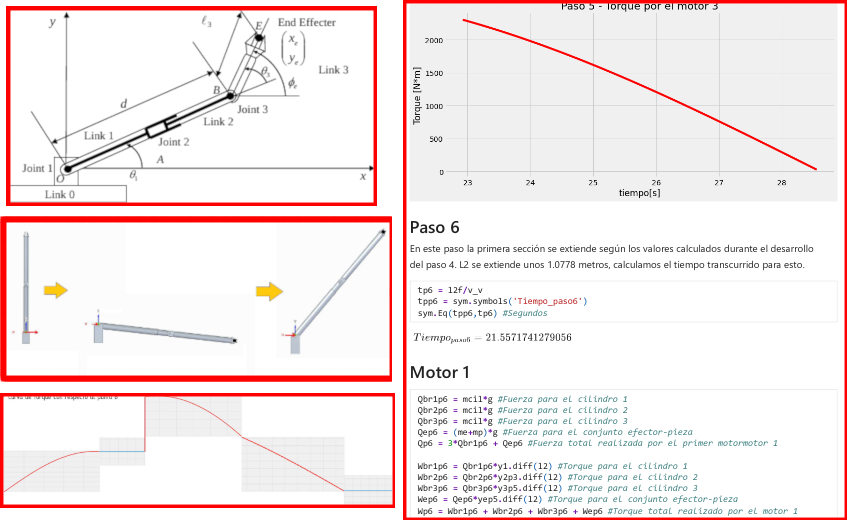
\includegraphics[width= \textwidth]{../figuras/robotArm.png}
	\caption{Ejemplo de un dispositivo mecánico realista que se analiza en el curso de mecánica analítica.}
	\label{fig:ejemploDispositivo}
\end{figure}


\subsection{Resolver ejercicios con código es más compatible con la inteligencia artificial de los LLM}

El uso de inteligencia artificial en el ámbito educativo es algo inevitable en el presente, como lo es en el ámbito profesional de la ingeniería.
Las interfaces de conversación (chat) de grandes modelos de lenguaje en línea como ChatGPT de OpenAI, DeepSeek, GitHub Copilot o Google Gemini son herramientas a las que recurren los alumnos para resolver problemas de física, quieran los docentes o no que las utilicen.
El procedimiento que sigue un alumno de un curso tradicional involucra transcripciones desde y hacia el LLM.
En manera imperfecta escribe su avance en la resolución, o en el peor de los casos el enunciado completo, y nuevamente debe hacer lo propio al papel a partir de las respuestas que obtiene del LLM.
No queda registro público de la interacción alumno-LLM, pues esto queda como un asunto privado del primero.

En el curso de la UNLaM se hace explícita la sugerencia de apoyarse en los LLM para la resolución de los ejercicios al tiempo que se transmite la virtud de guardar registro de consultas (prompts) al LLM adjunto a cada sección correspondiente del código.
La resolución de problemas a través de código evita transcripciones equívocas, puesto que el LLM interpreta con más fidelidad el código que el texto escrito en lenguaje natural tratando de explicar ambigüedades del problema.
Los alumnos enfrentan así su solución asistiéndose de consultas al LLM que en contrapartida sugiere correcciones a su código, como muestra el ejemplo de la Figura \ref{fig:Gemini}.

\begin{figure}[ht]
	\centering
	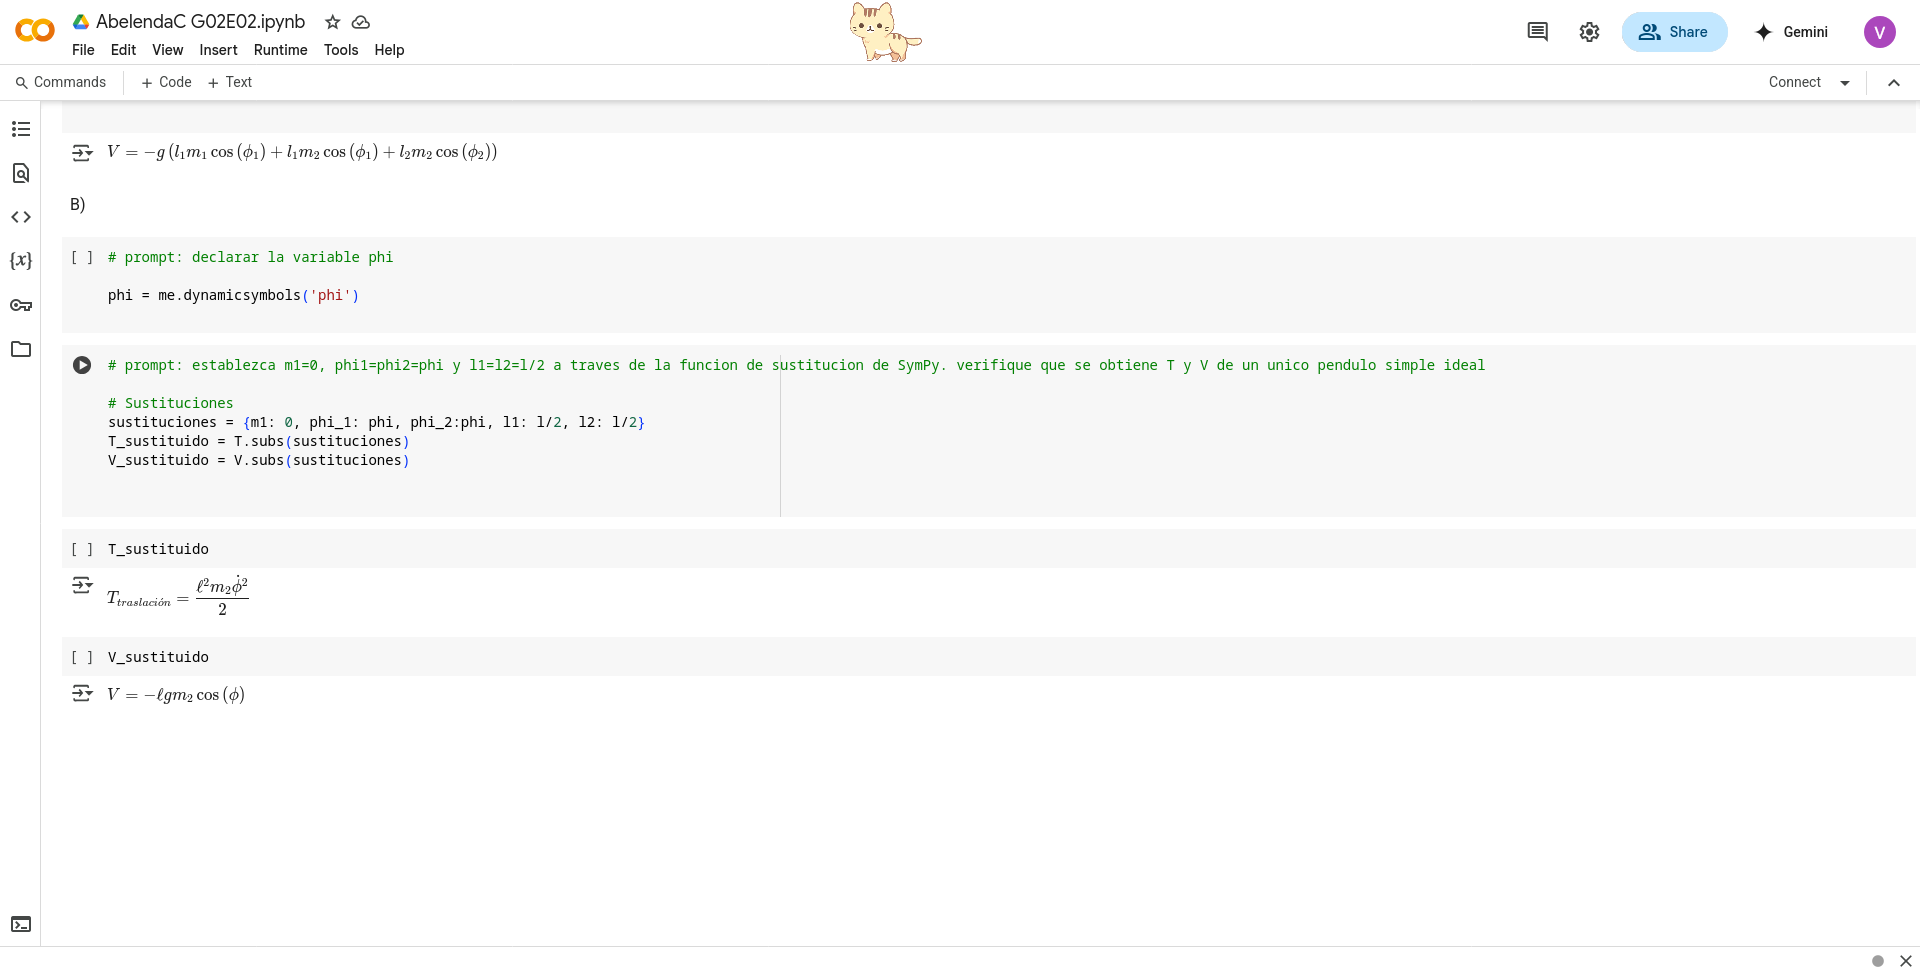
\includegraphics[width=\textwidth, trim={0 8cm 0 0},clip]{../figuras/gemini.png}
	% same as above but cropping the lower 1/4
	\caption{
		El alumno puede refinar su consulta (prompt) para cada bloque de código, aproximándose a la solución que busca.
		Aquí dejó constancia como comentario en el bloque de código del prompt que realizó al LLM Gemini de Google dentro de su cuaderno Jupyter ejecutado en el entorno Google Colaboratory.
		}
	\label{fig:Gemini}
\end{figure}

Cabe acotar que los docentes paulatinamente nos tornamos en orientadores sobre como guardar un sentido crítico hacia los resultados que arrojan las consultas a los LLM.
Se tuvieron cortas conversaciones con cada alumno sobre qué malinterpretaciones podrían estar sucediendo en ambos sentidos de su intercambio con el LLM. 

% \mr{acá tocás un punto adicional. No les estamos enseñando a les estudiantes a interactuar con los LLM correctamente y utilizarlos con mirada crítica. Por ejemplo, en el caso del problema del half-pipe, algunos lo metían en el LLM y éste asumía que el sistema era puntual, si no razonaban el resultado, no se daban cuenta del error. Tal vez sería importante incuir una línea de esto, se me ocurre algo en la línea de: Pero además, debemos oerientarles en tal sentido, es crítico que los docentes introduzcan estos sistemas y enseñen su uso y limitaciones.}
% No es realista pretender que puedan escindirse los LLM de los cursos de ingeniería de aquí en más.

% \mr{Incluiría algún párrafo en el orden de (modificalo o sacalo si no te cierra): Además, es deber del grupo docente entrenar a los estudiantes en este tipo de interacción, ya que el uso de LLMs se ha vuelto omnipresente. En el ejemplo expuesto se muestra el uso explícito para generar código, sin embargo fácilmente puede ser utlizado en infinidad de otros ámbitos, resolución directa del problema, generación de imágenes del problema, de presentaicones, de explicaciones. Pero en todos estos casos es fundamental enseñar cómo ser crítico sobre las respuestas que este tipo de sistemas nos otorgan.}

\subsection{Aula invertida: el docente debe ayudar con los ejercicios, no está para dar conferencias}

Una fuerte limitación que se enfrenta en la UNLaM es el limitado tiempo de clase.
Los alumnos en el estadio de cursada de la carrera de ingeniería mecánica en que se dicta el curso de mecánica analítica, suelen tener empleos de jornada completa.
Las escasas horas dentro de la semana se reparten en las diversas asignaturas haciendo que haya poco tiempo para un contacto sincrónico con el docente.  

El curso abordó esta cuestión creando un entorno de aprendizaje en línea y asíncrono que permite a los alumnos estudiar a su propio ritmo mediante el enfoque de aula invertida (flipped classroom) \cite{moraros_flipping_2015} que ilustra la Figura \ref{fig:flippedClassroomSchedule}.

\begin{figure}[ht]
	\centering
	\begin{subfigure}[b]{0.45\textwidth}
		\centering
		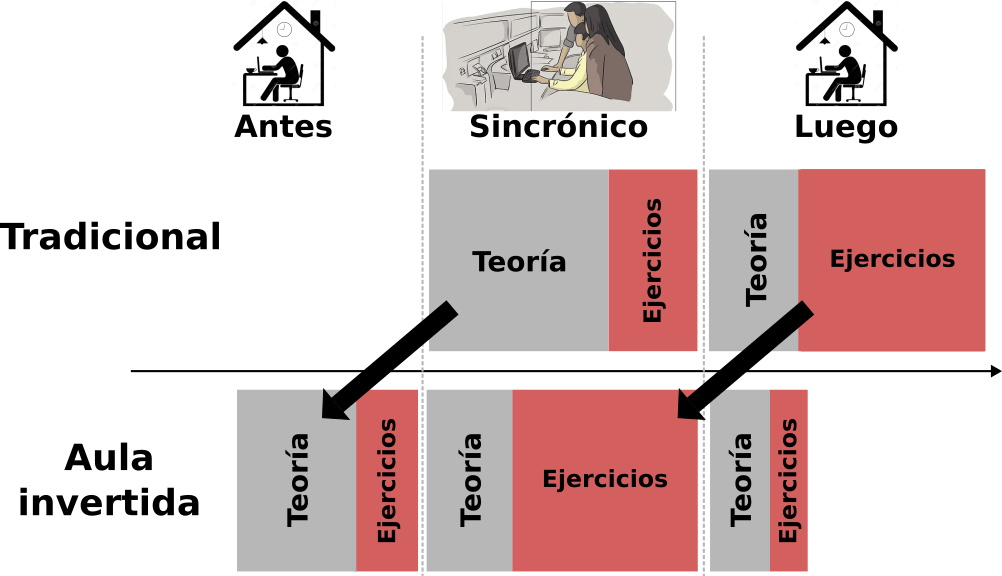
\includegraphics[width= 0.85\textwidth]{../figuras/flippedClassroomSchedule_castellano.png}
		\caption{El alumno lee e intenta aplicar nueva teoría antes del encuentro sincrónico con el docente.
		Este se reserva a resolver dudas y discutir los problemas que no se han podido resolver.}
		\label{fig:flippedClassroomSchedule}
	\end{subfigure}
	\hfill
	\begin{subfigure}[b]{0.5\textwidth}
		\centering
		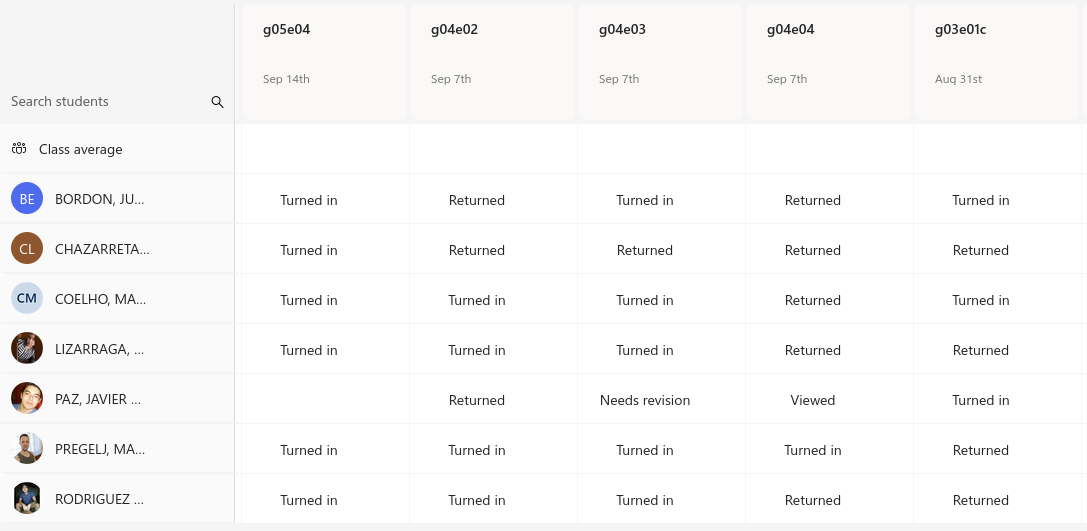
\includegraphics[width=0.9\textwidth]{../figuras/seguimiento.png}
		\caption{A través del sistema Microsoft Teams se lleva un control de entregas de todos los ejercicios de las guías y de su estado de corrección. A través del mismo los alumnos realizan consultas asincrónicas.}
		\label{fig:teams}
	\end{subfigure}
	\caption{La metodología de aula invertida se apoya en sistemas en línea.}
	\label{fig:flipped}
\end{figure}

Antes de las reuniones semanales, los alumnos deben estudiar la teoría y los ejemplos proporcionados en los cuadernos Jupyter, así como iniciar la resolución de los ejercicios que los acompañan.
Durante esas reuniones vespertinas, ya sean en línea o presenciales, se anima a los alumnos a que formulen preguntas y comenten con el profesorado los problemas que no hayan podido resolver.
Fuera de tal horario se hace uso de la plataforma Microsoft Teams para que los alumnos puedan realizar consultas asincrónicas al docente.
El docente accede a los cuadernos en Google Colaboratory, en el que puede realizar comentarios y correcciones directamente en la celda de código en cuestión donde corresponde hacerlos.
En Teams se hace un seguimiento de los ejercicios que los alumnos van entregando como resueltos en el formato de un enlace a sus copias personales de cuadernos de Jupyter, como ilustra la Figura \ref{fig:teams}.
Todos los ejercicios de las guías deben entregarse para la corrección, una tarea que está al alcance del tiempo disponible por el docente que está centrado en esta tarea, y en responder consultas, en vez de repetir todos los cuatrimestres idéntico soliloquio frente a un pizarrón.
La evaluación del aprendizaje parte de los registros de entrega de los mencionados ejercicios y la conversación que se tiene con los alumnos.
Unos pocos minutos de preguntas sobre como estos últimos implementaron una parte del código para resolver una parte específica del problema es tan o más reveladora sobre cuanto aprendió que un examen escrito.


% \section{CURSO DE ELECTROSTÁTICA ELEMENTAL}
\section{CURSO DE INTRODUCCIÓN A LA ELECTROSTÁTICA}

Las actividades descriptas en esta sección, que se están desarrollando en un curso de Física 2 de la Universidad Tecnológica Nacional - Facultad Regional Avellaneda (UTN FRA), están fuertemente inspiradas en el curso de mecánica analítica \cite{bettachini_CLADI_2022} presentado en la sección anterior. La principal diferencia con dicho curso de mecánica, además de los temas estudiados, es el nivel de avance en sus carreras de las y los estudiantes en sendos cursos. En la materia Física 2 nos encontramos con estudiantes que poseen pocos o nulos conocimientos tanto de programación como de cálculo numérico. Entonces, en este caso, es importante sostener como premisa que el código sea sólo una herramienta que asiste a una mejor adquisición de los conceptos de la materia impartida, y que la comprensión del código no se transforme en una dificultad extra. Con este objetivo, las numerosas e intrincadas líneas de código para cálculos complejos y generación de figuras, están encapsuladas en funciones de bibliotecas del paquete {\tt frautnEM} (\url{https://github.com/frautn/frautnEM}), diseñado específicamente para asistir a este curso, de forma que las y los estudiantes solo trabajen con pocas líneas de código sencillo. A su vez, el material que utilizan docentes y estudiantes de este curso está disponible para ser utilizado, descargado y adaptado libremente en el repositorio \url{https://github.com/frautn/F2-electromagnetismo}.\par\medskip

El material se presenta a las y los estudiantes dividido en módulos, mediante cuadernos Jupyter que se cargan en la plataforma Google Colaboratory, y que contienen breves explicaciones, ejemplos resueltos con código, y actividades propuestas para ser realizadas reutilizando el código de los ejemplos. Estos módulos asisten a estudiantes de un primer curso de electromagnetismo en la adquisición de conceptos sobre campo y potencial electrostático, distribuciones contínuas de carga, campo y equipotenciales en presencia de conductores, enteramente utilizando código Python. En poco tiempo se encuentran trabajando en ejercicios cuya resolución en papel está descartada, no necesariamente por su dificultad, sino también por el volumen de cálculos repetitivos que deberían ser realizados.\par\medskip

A modo de ejemplo, la Figura \ref{fig:anillo} muestra como las y los estudiantes generan líneas de campo de un anillo cargado con una distribución de carga no uniforme. La Figura \ref{fig:anillo}(a) es el código provisto con el cuaderno Jupyter para generar una lista de cargas puntuales que simulen una distribución contínua con forma de anillo. Copiando este código, el o la estudiante solo debe modificar la función que calcula la carga en cada ángulo, escribiéndola en un formato familiar, en este caso como {\tt a*cos(2*t)}, siendo {\tt t} el ángulo, el radio del anillo y el número de cargas puntuales utilizadas para representar al anillo.  

\textcolor{red}{Se analizan las líneas de campo y las equipotenciales de distribuciones de cargas arbitrarias, como la mostrada en la figura 1, o incluso visualizaciones en 3 dimensiones, tareas imposibles de implementar si se trabajara en papel. En la misma figura se destaca la simplicidad con la que los estudiantes pueden generar dichos gráficos, mediante el llamado a una única función diseñada específicamente para este curso. A lo largo de toda la experiencia, los estudiantes solo necesitan modificar códigos sencillos.}\par\medskip

Figura: Código simple que genera líneas de campo.




Ver Figura \ref{fig:anillo}.

\begin{figure}[h]
	\centering
	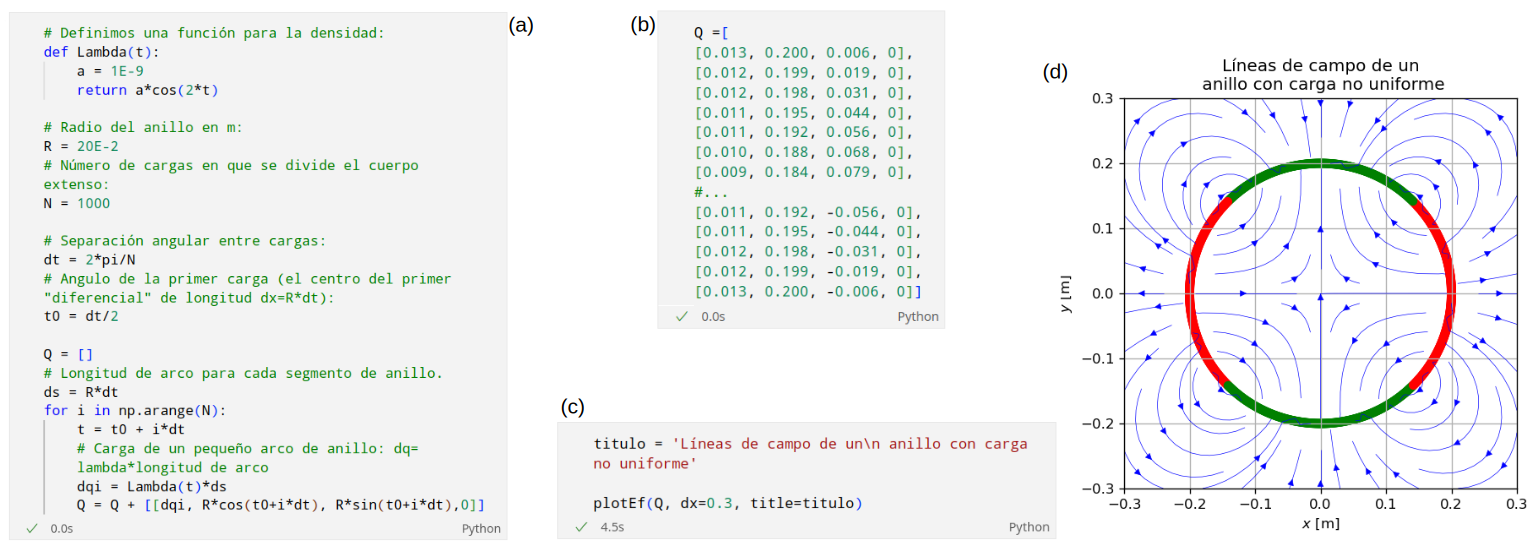
\includegraphics[width=160mm]{imagenes/anillo-variable.png}
	\caption{(a) Código para generar una lista de cargas puntuales que representen un anillo con carga variable. (b) La misma lista puede ser generada en una planilla de cálculo e ingresada manualmente. (c) Código muy breve y sencillo para generar las líneas de campo de esta distribución compleja. (d) La figura generada por la función {\tt plotEf()}.}
    \label{fig:anillo}
\end{figure}




Salir del plano. Ver Figura \ref{fig:superficies}.

\begin{figure}[h]
	\centering
	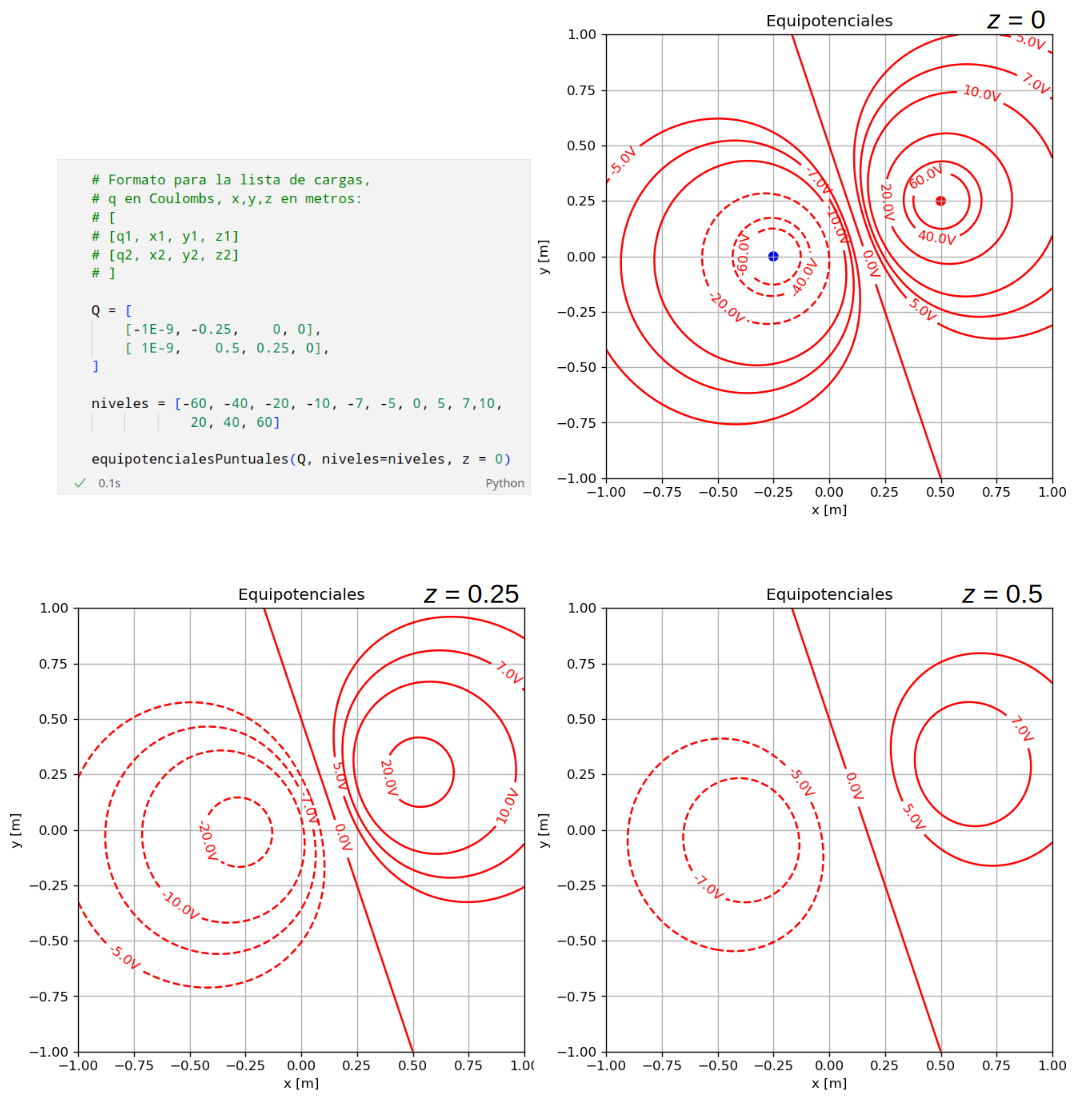
\includegraphics[width=160mm]{imagenes/equipotenciales_superficies.png}
	\caption{Con una simple línea de código se pueden estudiar las curvas equipotenciales resultantes de la intersección de las superficies equipotenciales con planos a diferentes alturas ($z = 0$ y $z = 0.5$) respecto de las cargas.}
    \label{fig:superficies}
\end{figure}

Con esta metodología, los estudiantes pueden:
\begin{itemize}
\item repasar lo trabajado en clases previas y adquirir nuevos conceptos sobre campo y potencial eléctrico;
\item acostumbrarse a que las distribuciones contínuas de carga eléctrica se pueden analizar como formadas por numerosas cargas puntuales, comprobando que se obtienen resultados muy aproximados a los resultados exactos que se obtienen usando fórmulas conocidas, como pueden ser la del campo eléctrico de esferas, líneas o planos cargados;
\item \textcolor{blue}{no trabarse con integrales que no dominan: más problemas en menos tiempo, más práctica para incorporación de conceptos, velocidad y facilidad para analizar variando parámetros;} 
\item reutilizar y adaptar código para experimentar con problemas cada vez más complejos, incluso no solo entre los propuestos en esta materia, sirviendo como una herramienta que se pueda aprovechar en otros contextos.
\end{itemize}
 
En el caso de los docentes, entre sus posibilidades se encuentran:
\begin{itemize}
    \item incluir en sus propuestas la resolución y el análisis de problemas que suelen estar descartados en una clase de pizarrón, debido a la dificultad de su abordaje (como es el caso del trabajo en 3 dimensiones) o a la longitud de los cálculos, aprovechando la reutilización de código;
	\item no destinar excesivo tiempo (de docentes y de estudiantes) repitiendo cálculos pesados, como por ejemplo las integrales múltiples relacionadas a distribuciones contínuas de cargas, y destinar ese tiempo al análisis de un mayor número de situaciones.
\end{itemize}


\textcolor{red}{Módulo 6 - Trabajo final: Se pide la resolución de un problema que involucre más de una de las herramientas usadas anteriormente, y se provee un cuaderno Jupyter en forma de plantilla para facilitar el inicio del trabajo.}

Extra: Aprovechar las posibilidades de cálculo simbólico que provee la biblioteca SymPy (Meurer et al., 2017) de Python para obtener soluciones exactas a problemas que involucran integrales múltiples complicadas y herramientas de análisis que aún no manejan.\par
\textcolor{red}{Módulo 4 - Distribuciones de carga contínuas (parte 2): Se obtienen soluciones exactas de configuraciones con distribuciones contínuas, utilizando la biblioteca Sympy para el cálculo de las integrales y los gradientes. En la figura 2 se muestra a modo de ejemplo el cálculo del campo generado por un segmento de carga. Notar que se obtiene el resultado del campo en cualquier posición, no solo en los ejes de simetría, que es una limitación usual al trabajar en papel.}\par
Conductores, simulación de la práctica de laboratorio.\par
\textcolor{red}{Módulo 5 - Campos y equipotenciales en presencia de conductores: La teoría involucrada para obtener equipotenciales cuando se tienen conductores con carga superficial no uniformes no forma parte de un curso de este nivel. Sin embargo, el análisis de los resultados sí puede incluirse como tarea. En particular, en este curso en el cual se está llevando a cabo la experiencia, los estudiantes realizan una práctica de laboratorio donde mapean el voltaje en una cuba que contiene electrodos extensos mantenidos a potencial constante, para luego estimar las curvas equipotenciales y las líneas de campo correspondientes. Por lo tanto, los análisis que los estudiantes realicen en este módulo son muy similares a dicha tarea de laboratorio. El código necesario para generar los gráficos está esencialmente provisto en bibiliotecas, por lo que los estudiantes sólo deben familiarizarse con la forma de presentar la geometría de los conductores.}\par\medskip  

Conclusiones:\par

“Since the notebooks are interactive, students can change the values of variables in an equation and immediately see what happens. That gives them a better sense of the physical reality underlying the equations,” 



\section{RESULTADOS}

En ambos cursos, los docentes fuimos capaces de proponer la resolución y el análisis de problemas que suelen estar descartados en una clase de pizarrón, debido a la dificultad de su abordaje.
La reutilización de código, evitó destinar un tiempo excesivo a la repetición de cálculos extensos, e.g. los involucrados en las integrales múltiples para distribuciones continuas de cargas del curso de electromagnetismo, o aquellos de fuerzas de ligadura en sistemas de múltiples cuerpos del curso de mecánica analítica.
Se observó que los estudiantes repasaron en un mayor número de situaciones lo trabajado en clases previas y sobre nuevos conceptos de una complejidad que excede a lo que usualmente se puede trabajar en el pizarrón.
Concurrentemente, se constató una retroalimentación más rápida, lo que facilitó una estrategia de prueba y error para confirmar o corregir sus soluciones.

Los estudiantes de electromagnetismo constataron resultados de fórmulas para distribuciones continuas de carga con los cálculos que realizaron con numerosas cargas infinitesimales.
Adaptando el código provisto pudieron responder preguntas de un trabajo final que no podrían haber resuelto en papel durante una clase tradicional. 
% En particular, las preguntas del trabajo final no se podrían haber resuelto en papel durante una clase tradicional, y, sin embargo, los seis grupos, de dos o tres integrantes, que participaron de la experiencia, pudieron responder satisfactoriamente a las preguntas adaptando el código provisto.



% ------------------------------------------------------------------------------
\section{CONCLUSIONES}
%Se apreciará que las mismas evidencien solidez y coherencia. Pueden incluirse en ellas otras cuestiones, como, por ejemplo, mención de interrogantes no dilucidados que podrían ser abordados en el futuro.

La naturaleza interactiva de los cuadernos Jupyter permitió a los alumnos adquirir una mejor comprensión de la física detrás de las ecuaciones, modificando parámetros y obteniendo resultados inmediatamente, resultados que son correctos y no dependientes de sus habilidades matemáticas.
% Gracias a la naturaleza interactiva de los cuadernos Jupyter, se comprobó durante las actividades en clase que las y los estudiantes adquieren una mejor comprensión de la física detrás de las ecuaciones, modificando parámetros y obteniendo resultados inmediatamente, resultados que son correctos y no dependientes de sus habilidades matemáticas.\par\medskip
La herramienta permitió evitó restringirse a problemas extremadamente sencillos o con aproximaciones exageradas, que pueden cimentar conceptos erróneos.
Asimismo hace de las herramientas enseñadas en asignaturas de física algo aplicable a situaciones más realistas habilitando al alumno a comprobar reglas de ingeniería que aprenderá en posteriores asignaturas de la carrera.

% ESTO YA LO DECIMOS EN LA INTRODUCCIÓN
%La resolución de ejercicios en cursos introductorios en ingeniería suele restringirse a problemas extremadamente sencillos o con aproximaciones muchas veces exageradas.
%Sin embargo, el análisis de los resultados de situaciones más complejas resulta valioso, evitando aproximaciones exageradas que no solo pueden formar conceptos erróneos, sino hacer de las herramientas de las asignaturas de física algo que no se puede aplicar a situaciones reales.

En el curso de mecánica analítica se modelizó y analizó la dinámica de dispositivos mecánicos realistas, que no podrían haber abordado en una clase tradicional.
Se está incorporando cuadernos Jupyter para el análisis de vibraciones, para que el alumno cuente con herramientas para encarar problemas de elementos de máquinas y estabilidad de estructuras apenas inicie la cursada de las asignaturas correspondientes.

En el curso de electromagnetismo, se planea incluir un módulo con ejercicios de campos y equipotenciales en presencia de conductores.
En particular, se incluirá el análisis numérico de una práctica de laboratorio donde se mapea el voltaje en una cuba que contiene electrodos extensos mantenidos a potencial constante, donde las y los estudiantes solo deberán describir la geometría de los conductores mediante funciones matemáticas sencillas.
% \textcolor{red}{(incluir una referencia, un link a la guía de laboratorio publicada en internet, al cuaderno jupyter para este análisis, footnote, o nada?)}
% NADA....
Asimismo, se planea registrar cada intento de resolución de problemas de los estudiantes, no solo el resultado.
Gracias a la utilización de un paquete de funciones propio, se guardará registro de los parámetros cada vez que los estudiantes ejecuten las funciones, habilitando un análisis de sus estrategias de resolución y procesos deductivos.

% ------------------------------------------------------------------------------
\section{AGRADECIMIENTOS}
% Adicionalmente, puede incluirse un apartado dedicado a los agradecimientos a personas o instituciones que han contribuido para la realización y/o financiación del trabajo.

Los autores desean agradecer al DIIT de la UNLaM por su apoyo a través de los proyectos C2-ING-109 (2023-2024) y C2-ING-143 (2025-2026).
Este último es parte del Programa de Investigación Mejora de las Estrategias Pedagógicas dirigido por la Dra. Bettina Donadelllo.
Ambos proyectos están acreditados en el Programa de Investigación Científica, Desarrollo y Transferencia de Tecnología e Innovaciones (CyTMA2) del DIIT.


% -----------------------------------------------------------------------------	
% \section{REFERENCIAS}

%Se considera valioso incluir menciones a textos y artículos de publicaciones reconocidas, valorándose la incorporación de aquellas de reciente edición. La forma de indicar las citas bibliográficas en el texto está especificada al final de la sección \textbf{1. INTRODUCCIÓN}. Solamente deben incluirse las referencias citadas en el cuerpo del documento, según su orden de aparición. El formato de las referencias según \textbf{Normas APA (7ª edición, 2024)}. A continuación, se brindan algunos ejemplos:
%
%\textbf{1. Libro} \cite{budynas_diseno_2012}
%
%[1] Apellido, A. A. y Apellido, B.B. (Año). Título del libro en cursiva. Edición. Editorial.
%
%\textit{\textbf{Ejemplo:}}
%\begin{enumerate}[label={[}\arabic*{]}]
%	\item Budynas, R.G. and Nisbett, J. K.  (2012). \textit{Shigley's Mechanical Engineering Design}. 9th Ed. McGraw-Hill.
%\end{enumerate}
%
%\textbf{2. Artículo de revista} \cite{moreno_abandono_2019}
%
%[2] Apellido, A.A. y Apellido, B.B. (Año). Título del artículo. Título de la revista en cursiva, volumen(número), páginas. https://doi.org/xxxx (si está disponible).
%
%\textit{\textbf{Ejemplo:}}
%\begin{enumerate}[label={[}\arabic*{]}]
%	\setcounter{enumi}{1}
%	\item Moreno J. and Chiecher A., (2019). \textit{Dropout in Engineering careers. A study of academic, socio-demographic, labor and life aspects}. Educational Research Notebooks, 10, (2),73-90, DOI:\\ https://doi.org/10.18861/cied.2019.10.2.2908
%\end{enumerate}
%
%
%\textbf{3. Artículo en línea} \cite{lu_aprobarias_2015}
%
%[3] Apellido, A. A. (Año). Título del artículo. Nombre del sitio web. URL
%
%\textit{\textbf{Ejemplo:}}
%\begin{enumerate}[label={[}\arabic*{]}]
%	\setcounter{enumi}{2}
%	\item Lu S. and Whiteman H. (2015) \textit{¿Would you pass the college entrance exam in China?}, CNN in espanish.\\
%	https://cnnespanol.cnn.com/2015/06/09/aprobarias-el-examen-de-ingreso-a-la-universidad-en-china
%\end{enumerate}
%
%\textbf{4. Informe o documento institucional} \cite{organizacion_mundial_de_la_salud_informe_2020}
%
%[4] Nombre de la institución. (Año). Título del informe en cursiva. URL (si aplica)
%
%\textit{\textbf{Ejemplo:}}
%\begin{enumerate}[label={[}\arabic*{]}]
%	\setcounter{enumi}{3}
%	\item World Health Organization. (2020). \textit{The World Mental Health Report}.\\
%	https://www.who.int/informes/saludmental2020
%\end{enumerate}
%
%\textbf{5. Tesis o disertación} \cite{jerez_resultados_2012}
%
%[5] Apellido, A. A. (Año). Título de la tesis o disertación en cursiva (Tesis doctoral, Nombre de la Institución que otorga el título). Nombre de la base de datos. URL (si está disponible)
%
%\textit{\textbf{Ejemplo:}}
%\begin{enumerate}[label={[}\arabic*{]}]
%	\setcounter{enumi}{4}
%	\item Jerez, O., (2012), \textit{Los resultados de aprendizaje en la Educación Superior por Competencias}. Doctoral Thesis, University of Granada, Spain. ISSN: 978-84-695.1027-8. https://dialnet.unirioja.es/servlet/tesis?codigo=62470
%\end{enumerate}
%
%\textbf{6. Norma o estándar} \cite{noauthor_iso_2020}
%
%[6] Nombre del organismo. (Año). Título de la norma en cursiva (Código y número de la norma). Editorial (si aplica). URL (si se obtuvo en línea).
%
%\textit{\textbf{Ejemplo:}}
%\begin{enumerate}[label={[}\arabic*{]}]
%	\setcounter{enumi}{5}
%	\item International Organization for Standardization. (2020). ISO 9001:2015: \textit{Sistemas de gestión de la calidad (Norma Internacional 9001)}.
%\end{enumerate}	
%
%\textbf{7. Trabajo presentado en un congreso o conferencia} \cite{xiaobin_stress_2013}
%
%[7] Apellido, A. A., y Apellido, N. T. (Año). Título del trabajo. Denominación del Congreso, Registro (ISBN o ISSN), Lugar y fechas.
%
%\textit{\textbf{Ejemplo:}}
%\begin{enumerate}[label={[}\arabic*{]}]
%	\setcounter{enumi}{6}
%	\item Xiaobin L. y Zelong L. (2013). \textit{Stress concentration factors due to typical geometric discontinuities for shaft design by numerical simulation}. ASEE Annual Conference and Exposition, Atlanta, Georgia, June 23-26, 2013, DOI 10.18260/1-2—22476 
%\end{enumerate}
%
%{\color{gray} \rule{\linewidth}{0.5pt}}
%\textbf{Pautas importantes:}
%\begin{itemize}
%	\item \textbf{Cursiva}: Los títulos de libros y de revistas, denominación de congreso y normas deben ir en cursiva.
%	\item \textbf{DOI}: Si un artículo tiene un DOI, debe incluirse al final de la referencia.
%	\item \textbf{URL}: En el caso de las fuentes en línea, incluye la URL completa, con texto en color negro sin formato de hipervínculo. No aplica ``Recuperado de'' a menos que sea necesario (por ejemplo, si la fecha de acceso es relevante).
%\end{itemize}
%
% ------------------------------------------------------------------------------
\renewcommand{\refname}{REFERENCIAS}% cambio de nombre
% \renewcommand{\bibname}{Referencias}% cambio de nombre
%\nocite{*}
\printbibliography


\end{document}

% ##############################################################################
% ##############################################################################